%%%%%%%%%%%%%%%%%%%%%%%%%%%%%%%%%%%%%%%%%%%%%%%%%%%%%%%%%%%%%%%%%%
\section{Simulación de las topologías en \acrshort{den2ne}}

Esta Sección viene dada por el objetivo de obtener el conjunto de datos final sobre el que se entrenarán los modelos de \gls{ml} en el Capítulo \ref{cha:desarrollo}. Para lograrlo, se necesita emplear el algoritmo \gls{den2ne} para realizar un gran número de simulaciones a partir de las topologías generadas en la herramienta \gls{brite} (ver Sección \ref{sec:ejebrite}). 

\vspace{3mm}

En primera instancia, es imprescindible implementar una serie de modificaciones en el algoritmo \gls{den2ne} para ajustar su funcionamiento al requerido para obtener el dataset final. La secuencia de acciones que se llevará a cabo se detallará en la Sección \ref{sec:cambiosden2ne}. Es importante indicar que es en este punto donde se introducirán las cargas netas resultantes de haber combinado los datos de consumo y de producción en la etapa de procesamiento (ver Sección \ref{sec:combinacion}). De la misma forma, se detallará el método de determinación de errores en las pruebas que servirá de base para después entrenar los modelos de \gls{ml}.

\vspace{3mm}

Por consiguiente, se añade la Sección \ref{sec:confden2ne} donde se especificará cómo se configurarán los parámetros de entrada requeridos para lanzar múltiples simulaciones. Además, se cuantificará el número total de pruebas posibles que se podrían llegar a realizar a partir de la información procesada y de las topologías generadas. 

\vspace{3mm}

Se comprobará a través de diferentes pruebas que los cambios introducidos en el algoritmo \gls{den2ne} producen una operativa acorde a las necesidades de este \gls{tfm}. Por último, a partir de los resultados obtenidos en las simulaciones, se concluirá con la Sección \ref{sec:datasetfinal} para exponer las características del dataset final que se utilizará para el entrenamiento de los modelos.




\subsection{Adaptación del algoritmo \acrshort{den2ne} a las pruebas}
\label{sec:cambiosden2ne}





\subsubsection{Cargas y simtest}
\label{sec:simtest}
%esto lo meto aqui temporalmente para poder poner la referencia abajo

%aquí va loadsamples.ipynb

% En otros términos, a partir de la selección de un instante temporal determinado en las pruebas, se aplicará uno de los 23 perfiles de carga disponibles de forma aleatoria a cada uno de los nodos que constituyen cada una de las topologías a probar.



\begin{figure}[H]
    \centering
    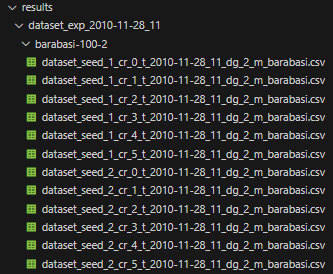
\includegraphics[width=0.55\textwidth]{img/diseno/dirpruebas.png}
    \caption{nomenclatura de los directorios y ficheros de resultados}
    \label{fig:dirpruebas}
\end{figure}





\subsection{Configuración de los parámetros de entrada}
\label{sec:confden2ne}

Para ejecutar \gls{den2ne}, es preciso definir la configuración de los parámetros de entrada en el script \textit{auto\_run.sh}. En la Sección \ref{sec:den2ne} se detallaba que este script se había diseñado con el objetivo de automatizar las simulaciones en el algoritmo y, como se ha expuesto en la Sección \ref{sec:cambiosden2ne}, ha sido necesario ajustar el mismo a los requerimientos de las pruebas de este \gls{tfm}. En este punto, se puede expresar que el cálculo de la cantidad total de configuraciones que se podrían llegar a realizar en \gls{den2ne} viene dado por el producto del siguiente conjunto de características:

\begin{itemize}
    \item El número total de topologías generadas: En la Sección \ref{sec:gentopo} se especifica una cantidad total de 180 topologías obtenidas a la salida de la herramienta \gls{brite}.
    \item El número de instantes temporales del dataset: El conjunto de datos resultante de la etapa de procesamiento, detallado en la Sección \ref{sec:combinacion} y, específicamente, en la Tabla \ref{tab:datacombinacion}, abarca una cantidad de filas igual al total de instantes temporales que se han tomado en consideración. En otros términos, al tratarse de muestras tomadas cada hora durante un rango temporal que comprende un año completo, su valor se calcula como 24x365=8760 instantes.
    \item El número de criterios: Como se detallaba en la Sección \ref{sec:den2ne}, \gls{den2ne} presenta 6 criterios de selección de los mejores caminos hacia el nodo raíz. En este caso, se implementan a las pruebas los 6 tipos.
    \item El número de tipos de escenarios de red: En la Sección \ref{sec:den2ne}, también se exponían los 4 tipos de escenarios que permite configurar el algoritmo. Teniendo en cuenta que las simulaciones deben acercarse a un entorno de \gls{sg} real y que el objetivo se basa en encontrar las transacciones energéticas entre nodos que superen la capacidad del enlace, se determina únicamente el escenario de pérdidas y límite de capacidad.
    \item Modo de limitación de carga: Se especifica únicamente el modo que determina valores de carga ilimitados.
    \item El número de semillas de ejecución: De la misma manera que se ha especificado anteriormente para \gls{brite} (ver Sección \ref{sec:conftopo}), se aplica al algoritmo \gls{den2ne} un conjunto de archivos de semillas para obtener simulaciones diferentes a partir de una misma topología a la entrada. En este caso, debido a la cantidad de datos que ya se maneja y para no introducir latencias considerables en el lanzamiento de las pruebas, se especifican 5 semillas por topología.
\end{itemize}

Por otro lado, en el caso de los parámetros de entrada referentes a las topologías, como son el número de nodos por topología, los modelos a simular y el número de semillas de generación, se sigue la misma configuración especificada en la ejecución de \gls{brite} (ver Sección \ref{sec:conftopo}). No obstante, para el grado de conectividad se determinan directamente los valores reales, suponiendo enlaces bidireccionales.

\vspace{3mm}

\begin{lstlisting}[language=bash, style=Consola, caption={Configuración de los parámetros de entrada en el script de automatización de \acrshort{den2ne}}]
TOPO_CRITERIONS=(0 1 2 3 4 5) # Criterios de selección de IDs
TOPO_BEHAVIORAL=3 # Tipo de escenario de red = modo Losses and Capacity (3)         
TOPO_LOAD_LIMIT=0 # Sin limite de carga
TOPO_RUNS=5 # Seeds de ejecución de DEN2NE

TOPO_NAMES=('barabasi' 'waxman') # Empleo de modelos RTWaxman y RTBarabasi (igual que BRITE)
TOPO_NUM_NODES=$(seq 100 50 200) # Número de nodos por topología (igual que BRITE)
TOPO_DEGREES=(2 4 6) # El grado de conectividad real (en BRITE 1, 2, 3)
TOPO_SEEDS=(1 2 3 4 5 6 7 8 9 10) # Seeds de generación de BRITE
\end{lstlisting}

\vspace{3mm}

Por tanto, teniendo en cuenta la configuración implementada para los parámetros de entrada, se puede determinar el número total de simulaciones únicas posibles a partir de la siguiente expresión:

    \[\textit{Nsim} = \textit{Ntopos} \times \textit{Ninstantes} \times \textit{Ncriterios} 
    \times \textit{Nescenarios} \times \textit{NNlimit} \times \textit{Nsem\_ejec}\]
    \[\textit{Nsim} = 180 \times 8760 \times 6 \times 1 \times 1 \times 5 = 47304000\] 












\subsection{Creación del dataset final y conclusiones de las pruebas}
\label{sec:datasetfinal}

%AQUI INTRO, 

%formato nomenclatura, comentar division de ficheros y directorios


  

%nombrar tabla final del procesamiento \ref{tab:datacombinacion} 

%agrupación de ficheros en datafinal.ipynb

Teniendo en cuenta lo anterior, se decide crear un nuevo \textit{notebook}, \textit{datafinal.ipynb}, con el fin de conseguir a la salida un conjunto de datos final por cada instante temporal especificado en las pruebas. Como se podía apreciar en la Figura \ref{fig:dirpruebas}, cada experimento creaba un directorio con la fecha y hora determinadas (ej. \textit{dataset\_exp\_2011-04-28\_11}) y, en su interior, se generaban los diferentes ficheros de resultados, organizados por carpetas en función del modelo y el grado de conectividad al que hacían referencia (ej. \textit{barabasi-200-6}). 

\vspace{3mm}

Por ello, a modo de simplificar el tratamiento de los resultados del algoritmo, el primer paso que se implementa en el \textit{notebook} se basa en el agrupamiento en un mismo \textit{dataframe} de todos los ficheros que se han generado para un instante determinado. Después, es importante comprobar que el porcentaje total de error u \textit{overflow} dado para el instante en cuestión no es nulo. Es decir, para cada instante temporal que se pruebe, se debe conseguir un conjunto de datos que contenga algunas filas el valor \textit{overflow} activo para después, entrenar de forma precisa los modelos de \gls{ml} y poder predecir cuándo se producirán estos errores.

\vspace{3mm}

%%%%%REVISAR!!!!!!!!!!!!!!!!!!!!!!!!!!!
El siguiente paso consiste en combinar los datos obtenidos de los resultados con la información de las viviendas aportada en el fichero de test. Es importante recordar que este fichero de test (ej. \textit{test\_2010-11-28\_11.csv}) se creaba a partir de filtrar en el dataset resultante del procesamiento las medidas de las viviendas para un instante temporal determinado y se aplicaba a la entrada de \gls{den2ne} para definir los valores de carga (ver Sección \ref{sec:simtest}). Por ello, en este punto es combinar cada fila del \textit{dataframe} de resultados con la información real de cada vivienda en función del identificador del nodo al que se hace referencia. 

\vspace{3mm}

\begin{lstlisting}[style=Python, caption={Combinación de resultados y test}]
df_merged = pd.merge(df, df_sim, left_on='origen_id', right_on='iid', how='outer') # Operación de merge
\end{lstlisting}

\vspace{3mm}

Tras esta operación, el nuevo \textit{dataframe} se constituye por todas las columnas necesarias, aunque antes estas se deben revisar y eliminar si vienen replicadas, como ocurre en el caso del identificador y la fecha. 
Finalmente, se almacena el \textit{dataframe} limpio en un fichero con formato .csv, tratándose del dataset final que se empleará en la etapa de desarrollo. Este fichero contiene los campos definidos en la Tabla \ref{tab:datafinal} y sigue una nomenclatura formada por la marca de tiempo a la que hace referencia (ej. \textit{2010-12-28\_11.csv}). %%tabla para cada fecha

\vspace{3mm}

\begin{table}[h!]
    \centering
    \begin{tabular}{|c|c|c|}
    \hline
    \rowcolor[HTML]{AAAAAA} 
    \multicolumn{1}{|c|}{\cellcolor[HTML]{AAAAAA}Campo} & \multicolumn{1}{c|}{\cellcolor[HTML]{AAAAAA}Descripción} & Unidades \\ \hline
    \textit{timestamp} & Instante temporal de medida & datetime \\ \hline
    \textit{datetime} & Fecha del valor promedio & datetime \\ \hline
    \textit{H} & Hora del valor promedio & - \\ \hline
    \textit{overflow} & Etiqueta binaria de superación de carga & - \\ \hline
    \textit{cap} & Capacidad del enlace & kW \\ \hline
    \textit{load} & Carga neta (\textit{Dif}) & kW \\ \hline
    \textit{dist} & Distancia & m \\ \hline
    \textit{origen\_id} & Identificador de nodo origen & - \\ \hline
    \textit{dest\_id} & Identificador de nodo destino & - \\ \hline
    \textit{len\_origen\_tag} & Longitud de la etiqueta del nodo origen & - \\ \hline
    \textit{len\_dest\_tag} & Longitud de la etiqueta del nodo destino & - \\ \hline
    \textit{modelo} & Modelo de topología & - \\ \hline
    \textit{criterion} & Criterio de selección de IDs & - \\ \hline
    \textit{degree} & Grado de conectividad & - \\ \hline
    \textit{total\_balance} & Balance de carga global & - \\ \hline
    \textit{abs\_flux} & Flujo total de carga en el nodo raíz & - \\ \hline
    \textit{Diffuse Irradiance} & Índice de radiación difusa (\gls{dif}) & W/m2 \\ \hline
    \textit{Plane of Array Irradiance} & Índice de radiación en el plano del array (\acrshort{poa}) & W/m2 \\ \hline 
    \textit{Ambient Temperature} & Temperatura ambiente & C \\ \hline
    \textit{Cell Temperature} & Temperatura de las células solares & C \\ \hline
    \textit{DC Array Output} & Potencia de salida DC del array & W \\ \hline
    \textit{AC System Output} & Potencia de salida AC del sistema & W \\ \hline
    \textit{Pavg} & Potencia consumida & W \\ \hline
    \textit{Dif} & Carga neta calculada & W \\ \hline
    \end{tabular}  
    \caption{Dataset final obtenido por cada instante temporal probado en \acrshort{den2ne}}
    \label{tab:datafinal}
\end{table}

Con la obtención de este conjunto de datos se finaliza la etapa de diseño y, por ende, el presente Capítulo. A partir de los resultados obtenidos, se puede expresar de forma concluyente que se cumple el objetivo principal de generar el dataset final que suponga la base del entrenamiento y el desarrollo de los modelos de \gls{ml} que se plantearán en el Capítulo \ref{cha:desarrollo}. Adicionalmente, a modo de simplificar la compresión de la secuencia de acciones que se han llevado a cabo durante este Capítulo, se representa la Figura \ref{fig:total}. En el diagrama se exponen los ficheros creados en cada paso, el tratamiento de los datos y los procesos ejecutados.
  
\pagebreak

\begin{sidewaysfigure}
    \centering
    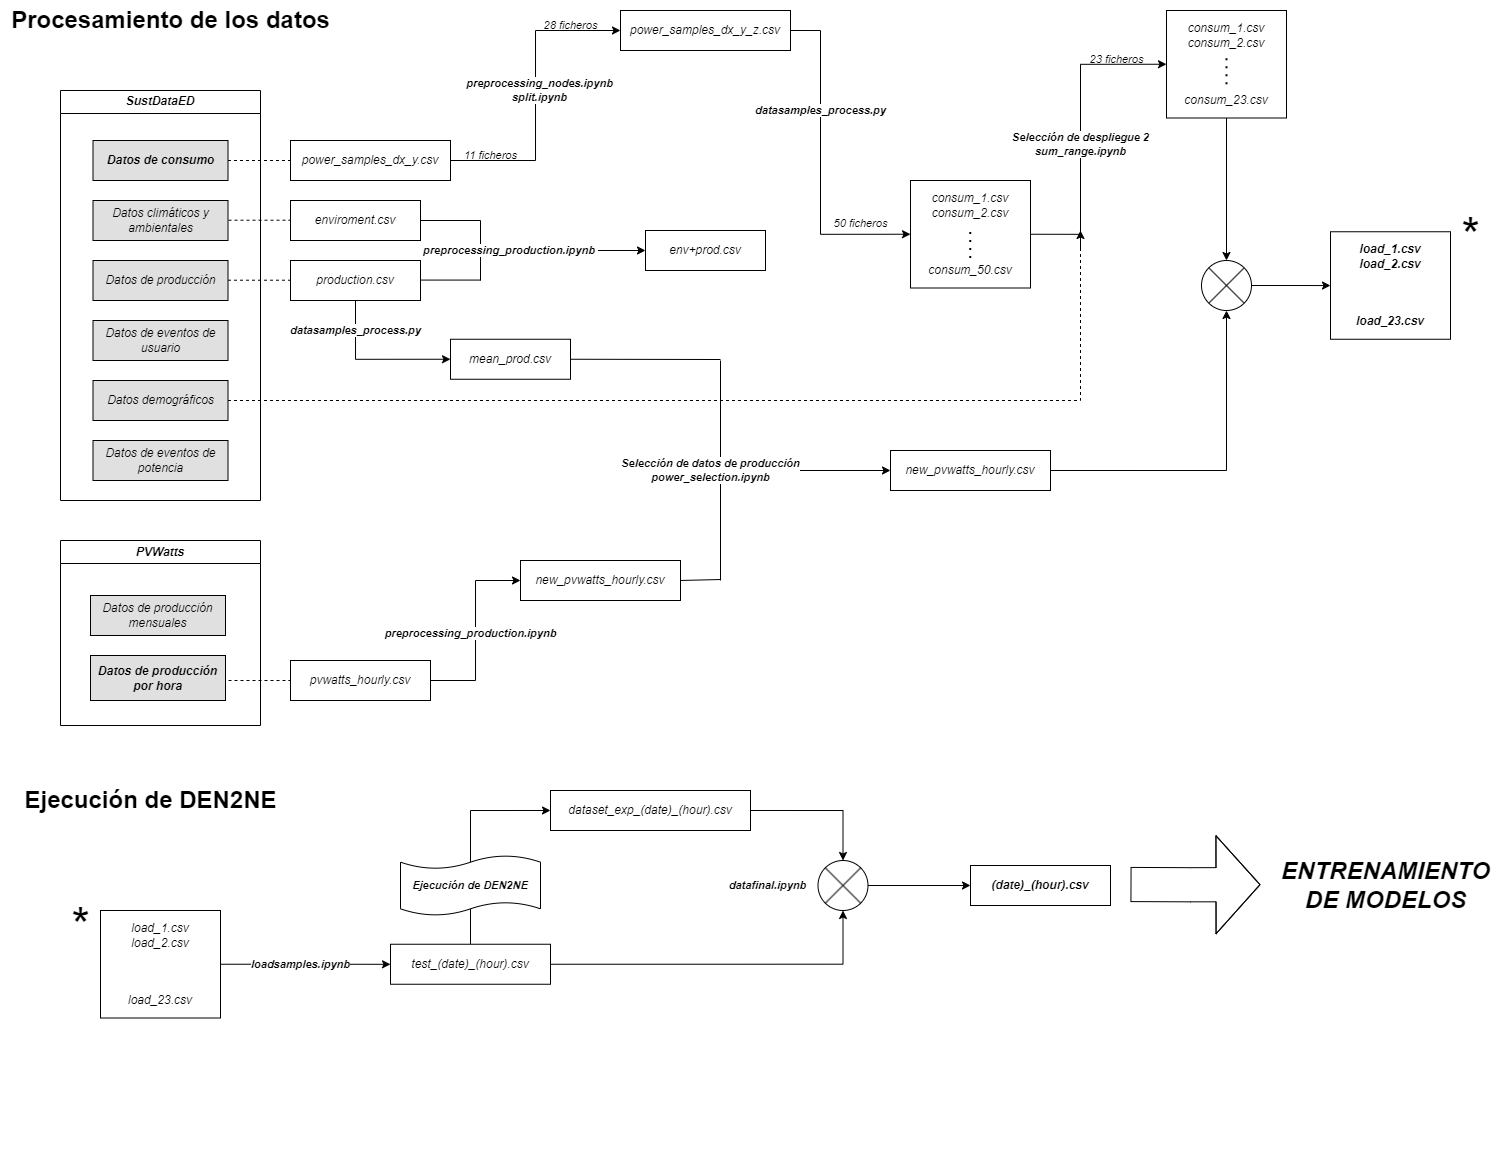
\includegraphics[width=1\textwidth]{img/diseno/total.png} 
    \caption{Diagrama completo de diseño del dataset final}
    \label{fig:total}
\end{sidewaysfigure}

